\documentclass[border=10pt]{standalone}
\usepackage{xcolor}
\usepackage{pgfplots}
\usepackage{tikz}
\begin{document}
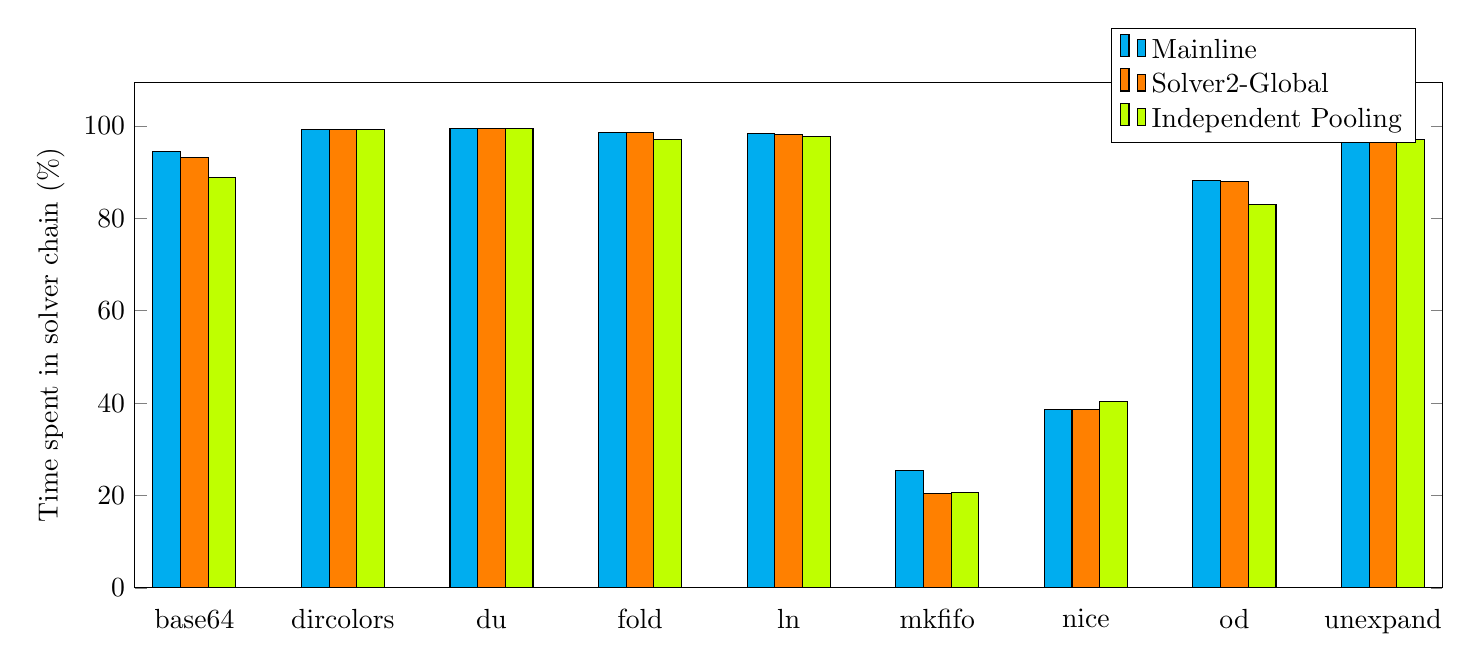
\begin{tikzpicture}
    \begin{axis}[
        width  = 1.5 * \textwidth,
        height = 8cm,
        major x tick style = transparent,
        % tickwidth=10,
        ybar=0,
        bar width=10pt,
        % ymajorgrids = true,
        ylabel = {Time spent in solver chain (\%)},
        symbolic x coords={base64,dircolors,du,fold,ln,mkfifo,nice,od,unexpand},
        xtick = data,
        scaled y ticks = false,
        enlarge x limits=0.05,
        ymin=0,
        legend cell align=left,
        legend style={
                at={(0.98,0.88)},
                anchor=south east,
                % column sep=1ex
        }
    ]
        \addplot[style={cyan,fill=cyan,mark=none}, draw=black]
	coordinates {(base64,94.44) (dircolors,99.19) (du,99.45) (fold,98.63) (ln,98.31) (mkfifo,25.34) (nice,38.57) (od,88.24) (unexpand,98.66)};
\addplot[style={orange,fill=orange,mark=none}, draw=black]
	coordinates {(base64,93.11) (dircolors,99.21) (du,99.38) (fold,98.66) (ln,98.18) (mkfifo,20.52) (nice,38.59) (od,87.89) (unexpand,98.65)};
\addplot[style={lime,fill=lime,mark=none}, draw=black]
	coordinates {(base64,88.90) (dircolors,99.24) (du,99.46) (fold,97.14) (ln,97.63) (mkfifo,20.64) (nice,40.44) (od,82.95) (unexpand,97.16)};

        \legend{Mainline,Solver2-Global,Independent Pooling}
    \end{axis}
\end{tikzpicture}
\end{document}
